% !TeX encoding = utf8
% !TeX program = xelatex
% -*- coding:utf-8 mod:LaTeX -*-

% Paper 5 — WCL (IEEE Wireless Communications Letters) version.
% Compressed from the frozen full-length IEEE Access manuscript
% (main.tex) — every number is taken from main.tex /
% paper5_task_oriented/EXPERIMENT_LOG.md; nothing new is measured here.
%
% v2 (2026-10-03/04): revision against the second external review
% (Major Revision).  Changes: decision-equivalence defined strictly
% (inference rule, not optimisation); oracle/diagnostic nature of the
% compensated receiver stated explicitly (detached phase alignment);
% direct output-SIR evidence for the interference-limited mechanism
% (analyze_sir_evidence.py -> results/sir_evidence.json, no new runs);
% 15 separators characterised; benchmark fully specified (less reliance
% on [9]); Table I gains mean±std and a formal Delta definition;
% "reward hacking" -> optimiser exploitation wording; S3 split into
% questions (A)/(B); conclusion claims layered and the final
% prescription softened; Fig. 1 uses the letter variant without the
% selection-biased recursive curve; [13] (6G semantic) removed; DOI
% TODO removed.
% v2 experiments (server, 2026-10-03/04, done): lambda_ser sweep
% {0.01,0.1,10} x 3 seeds (results/lambda_sweep/) and three additional
% test grids 100001-100003 (results/testseed_robustness*/), both folded
% into Sections II-IV; EXPERIMENT_LOG.md 2026-10-04 entry.

\documentclass[journal]{IEEEtran}

\usepackage{graphicx}
\usepackage{booktabs}
\usepackage{amsmath,amssymb}
\usepackage{url}
\usepackage{xcolor}
\usepackage[mode=text]{siunitx}
\sisetup{locale=US}
\usepackage{hyperref}
\hypersetup{hidelinks, colorlinks=true, allcolors=black,
  pdfstartview=Fit, breaklinks=true}

\newcommand{\snr}{\mathrm{SNR}}
\newcommand{\sir}{\mathrm{SIR}}

\begin{document}

\title{The Waveform-to-Bit Gap in Single-Channel Blind Source
Separation:\\A Decision-Equivalent Evaluation Protocol}

\author{Bin~Nong, Weihong~Fu, and Zhuoyun~Jiang%
\thanks{Manuscript prepared 2026. B.~Nong is with Tianfu College of
Southwestern University of Finance and Economics, Mianyang 621000, China
(e-mail: nongbin@tfswufe.edu.cn). W.~Fu is with the School of
Telecommunications Engineering, Xidian University, Xi'an 710071, China.
Z.~Jiang is with the School of Health Science and Engineering,
University of Shanghai for Science and Technology, Shanghai 200093,
China.}}

\markboth{IEEE Wireless Communications Letters, 2026}%
{Nong \MakeLowercase{\textit{et al.}}: The Waveform-to-Bit Gap in
Single-Channel Blind Source Separation}

\maketitle

\begin{abstract}
Separators for single-channel blind source separation (SC-BSS) of
co-frequency communication signals are trained and ranked by
waveform-fidelity metrics, yet the downstream task is demodulation.
This letter contributes a decision-equivalent evaluation protocol---a
diagnostic, oracle-compensated receiver whose hard decisions are
exactly reproduced by a differentiable soft receiver---and a
controlled five-seed study on a variable-count co-frequency benchmark.
The protocol exposes a large waveform-to-bit gap: $+4.1$\,dB of SI-SDR
improvement moves the compensated symbol error rate from 0.5049 to
0.5027, and direct output-SIR measurement shows why: separation
removes almost none of the interference ($+0.3$\,dB SIR gain at
$K{=}2$), the waveform gain being almost entirely noise-side. A
faithfully aligned task-oriented loss moves the pooled bit error rate
by at most 0.03 percentage points, but its sign is set by the number
of interferers: it helps at $K{=}2$ and hurts at $K{=}3$, cancelling
in the pool. A joint soft-information head fails at blind burst
synchronisation. The evidence suggests closing the gap requires
explicit receiver structure rather than re-weighting the tested task
loss.
\end{abstract}

\begin{IEEEkeywords}
Blind source separation, co-frequency communication, evaluation
protocol, symbol error rate, task-oriented learning.
\end{IEEEkeywords}

\section{Introduction}
\label{sec:intro}

\IEEEPARstart{S}{ingle-channel} blind source separation (SC-BSS) of
co-frequency communication signals---several modulated emitters
overlapping in time and frequency at one receiving antenna---has
progressed through a sequence of learned
separators~\cite{hou2022single,chen2019deep,ma2023novel,luo2023single,guo2024single},
trained and ranked by waveform-fidelity metrics, above all
scale-invariant SDR (SI-SDR)~\cite{kolbaek2017pit,leroux2019sdr}. Yet
separation is rarely the end goal: in spectrum monitoring and cognitive
radio, the separated waveforms feed a demodulator, and the quantity
paid for is the bit error rate (BER). The premise of the line of work
is that waveform fidelity is a good proxy for bit-level recoverability.
Audio research has shown such proxies can be
misleading~\cite{vincent2006bsseval,leroux2019sdr}; for co-frequency
\emph{communication} mixtures, where the task metric is sharp (symbol
and bit error rate), the premise has, to our knowledge, never been
tested under statistically controlled experiments.

This letter tests it. On the variable-$K$ co-frequency benchmark of our
companion open-world study~\cite{nong2026openworld}, we contribute: (i)
an \emph{offset-compensated diagnostic receiver} producing compensated
symbol error rate (SER) and Gray-mapped BER from shared decisions,
together with a differentiable soft-demodulation loss whose inference
rule is \emph{decision-equivalent} to it (identical argmax decisions),
so the training proxy and the evaluation truth are the same receiver
(Section~\ref{sec:protocol}); (ii) a controlled five-seed measurement
study showing the gap is real, structural, and interference-limited,
with direct output-SIR evidence for the mechanism
(Section~\ref{sec:exp}); and (iii) evidence that the prescription is
structural: closing the gap suggests explicit synchronisation,
equalisation and joint-detection
structure~\cite{verdu1998multiuser,dankberg1998pcma,andrews2005interference},
rather than re-weighting the tested task loss.

\section{Benchmark and Decision-Equivalent Protocol}
\label{sec:protocol}

The benchmark is unchanged from~\cite{nong2026openworld}; we restate
the parameters that matter for the protocol. A single complex mixture
$y(t) = \sum_{k=1}^{K} w_k s_k(t) + n(t)$, $t = 0,\dots,4095$ at
16\,kHz (256-symbol bursts, 16 samples/symbol, 1\,kBd), of
$K \in \{1,2,3\}$ sources drawn uniformly from
\{BPSK, QPSK, 8PSK, 16QAM\}, root-raised-cosine pulses (roll-off 0.35,
64-tap), an independent unit-norm 3-tap complex-Gaussian fading channel
per source, per-source carrier $2\,$kHz${}+\mathcal{U}(0,5)$\,Hz with
$\pm 5$\,Hz jitter, mixing weights $w_k \sim \mathcal{U}(0.4,0.6)$
unnormalised, giving a pairwise source-to-source SIR of
$\approx 0$\,dB by construction, and AWGN
with SNR defined on the total mixture power (per-source effective SNR
$= \snr - 10\log_{10}K$). The test grid is deterministic: 7 SNR points
($-10$ to $20$\,dB) $\times$ $K$, 100 mixtures per cell, seed 99999.

\emph{Evaluation truth.} The compensated receiver demodulates an
estimate--source pair as follows: both sides are down-converted at the
source's \emph{oracle} carrier (exposed by the generator), passed
through the RRC matched filter, sampled on the zero-delay symbol grid,
normalised to unit power, the estimate phase-aligned to the reference
by a single least-squares complex coefficient, and decided by
minimum-distance onto the constellation. Compensated SER is the
fraction of mismatched hard decisions; BER is defined post-hoc via a
Gray labelling of the constellation indices, from the \emph{same}
decisions. Pooled SER/BER are unweighted means over all matched
estimate--source pairs. Identity input scores SER $= 0.000$ for all
four modulations. We stress that this is a \emph{diagnostic instrument, not
a blind receiver}: by construction it factors synchronisation out of
the evaluation, isolating the waveform-fidelity$\,\to\,$symbol-decision
link that is the subject of this letter.

\emph{Decision-equivalent training proxy.} The soft receiver replaces
the hard decision by a cross-entropy over constellation points on the
same grid,
\begin{equation}
  \mathcal{L}_{\mathrm{soft\text{-}SER}}
  = -\frac{1}{N}\sum_{n}\log
  \frac{\exp(-|z_n - c_{\ell_n}|^2/\sigma^2)}
        {\sum_{m}\exp(-|z_n - c_m|^2/\sigma^2)},
  \label{eq:softser}
\end{equation}
with $z_n$ the aligned estimate's symbols, $\ell_n$ the reference's
hard decision, and $\sigma^2 = 0.1$ fixed on the unit-power symbol grid
across all experiments (not tuned). The alignment coefficient and the
labels $\ell_n$ are computed on detached tensors (stop-gradient), so
gradients flow only through the estimated waveform. Each logit is a
monotone transform of the negative squared distance, so its argmax
coincides with the minimum-distance decision for any $\sigma^2 > 0$ by
construction (additionally verified symbol-for-symbol on all four clean
modulations): the two receivers are decision-equivalent \emph{in their
inference rule}. The soft loss is
nonetheless a smooth relaxation of the hard count, so the equivalence
does not extend to the optimisation dynamics --- any effect it produces
is attributable to the task, not to a proxy mismatch.

\emph{Statistics.} All headline numbers are five-seed (42--46); the
primary test is the seed-level exact sign-flip permutation (power floor
$p = 0.0625$ at five seeds), with Bonferroni correction over the
pre-declared contrasts. Both headline findings below were additionally
replicated on three further deterministic test grids (seeds
100001--100003), so they reflect the mixture population rather than one
test realisation.

\section{A Decision-Level Reading}
\label{sec:reading}

The measurements below fall out of a simple observation. Write a
separated estimate of a target source $s$ as
\begin{equation}
  \hat{s} = \alpha s + \sum\nolimits_{j} \beta_j s_j + \nu ,
  \label{eq:decomp}
\end{equation}
with $s_j$ the co-channel interferers and $\nu$ the noise and artefact
residual. The compensated receiver normalises away the gain $\alpha$
and a constant phase, so its decisions depend on $\hat{s}$ only through
the symbol-grid SINR
$\gamma \triangleq |\alpha|^2 \big/
\big(\sum_j |\beta_j|^2 + \sigma_\nu^2\big)$ (unit-power sources).
Under a Gaussian approximation of the residual on the symbol grid, the
compensated SER is a non-increasing function of $\gamma$ alone: it is
invariant to any reallocation of residual energy between interference
and noise that preserves $\gamma$, and insensitive to reductions of
$\sigma_\nu^2$ while the interference term dominates. SI-SDR, in
contrast, weights the two terms equally. This has two consequences.

First, a separator whose SI-SDR gain is \emph{noise-side} leaves
$\gamma$ --- and hence the SER --- almost untouched at pairwise
$\sir \approx 0$\,dB, where $\gamma$ is saturated by the interference
term. The projection-power output SIR reported below is exactly the
interference factor of $1/\gamma$; it, not SI-SDR, is the
decision-relevant waveform metric, which is why we measure it directly.

Second, at pairwise $0$\,dB the observation constellation itself
overlaps: two equal-power in-phase BPSK sources coincide on the
decision boundary with probability $1/2$, an irreducible
$\tfrac{1}{4}$ error floor for that configuration that no noise
suppression can lower --- the collided symbol's label is simply not
present in the observation. The same label-ambiguity argument bounds
any decision-equivalent task loss: once this floor is reached, no
waveform-faithful descent direction remains, which is consistent both
with the sub-$0.05$\,pp weight sweep and with the off-manifold minima
the loss finds when the waveform anchor is removed
(Section~\ref{sec:exp}).

\begin{figure}[!t]
\centering
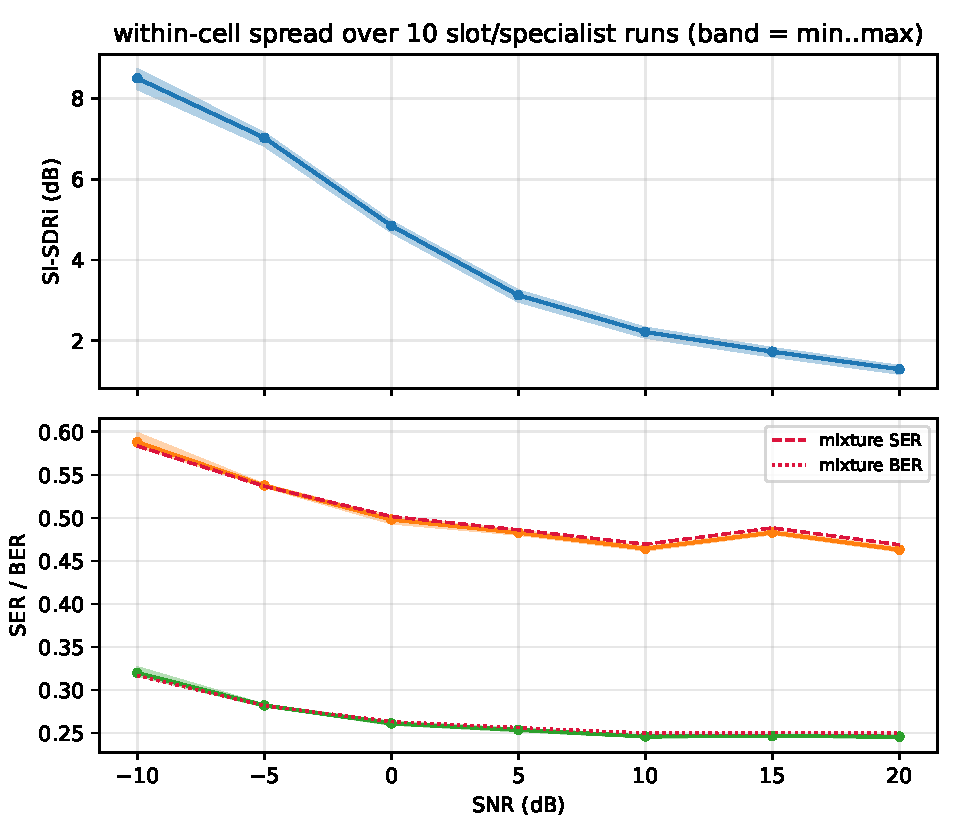
\includegraphics[width=\columnwidth]{figures/s1_flat_region_letter.pdf}
\caption{The waveform-to-bit gap. Top: SI-SDR improvement over the
mixture rises to $+8.4$\,dB at $-10$\,dB SNR (band: min--max over the
ten slot/specialist runs of the honest pool; the recursive variant is
excluded here because its 37\,\% miss rate makes its matched-pair SER
selection-biased). Bottom: the compensated SER/BER of the separated
outputs stays glued to the mixture baseline (dashed) at every SNR ---
the bits do not move.}
\label{fig:flat}
\end{figure}

\section{Experiments}
\label{sec:exp}

\emph{S1 --- the mismatch is real and large.} Fifteen previously
trained separators --- the three architectures
of~\cite{nong2026openworld} (slot, specialist-bank, recursive
one-and-rest), five training seeds each, all trained with the same
MSE-anchored waveform PIT loss on the same training distribution ---
improve SI-SDR by $+4.1$\,dB over the unseparated mixture on this
benchmark, but move the compensated SER from $0.5049$ (mixture, no
separation) to only $0.5027$ (BER $0.2669 \to 0.2651$); the per-SNR
improvement of $+8.4$\,dB at $-10$\,dB SNR buys nothing (a
fraction-of-a-point penalty, if anything) --- Fig.~\ref{fig:flat} shows
the whole curve. The damage localises to interference: the baseline
SER jumps from $0.146$ at $K{=}1$ to $0.561$ at $K{=}2$ and only
$0.587$ at $K{=}3$ --- one interferer closes nearly the whole
demodulation gap. Direct output-SIR measurement confirms the mechanism: with
$\sir(\hat{s}) = 10\log_{10}\big(p_t / \sum_{j \neq t} p_j\big)$, where
$p_j = |\langle \hat{s}, s_j \rangle|^2 / \|s_j\|^2$ is the projection
power of the estimate onto true source $j$, the per-source SIR is
$0.0$\,dB at the mixture input and only $+0.2$\,--\,$+0.3$\,dB after
separation at $K{=}2$, and $-3.1$\,dB at the input versus $-2.9$\,dB
after at $K{=}3$ --- the separators suppress noise and self-distortion
but pass the co-channel interferer almost untouched, and at
pairwise $\sir \approx 0$\,dB it is the interferer, not the noise, that
sets the decisions (the first consequence of
Section~\ref{sec:reading}: the gain is noise-side, so $\gamma$ and the
SER do not move). A fixed-$K{=}2$ SIR sweep shows the flatness persists to
input SIR $= 20$\,dB (gap to the per-cell baseline never exceeds $1$
percentage point and sign-flips), so the interference limitation is not
an artefact of the symmetric operating point. Nor is it an artefact of
the test grid: on three further independent test populations the
separated SER ($0.504$--$0.508$) stays glued to its mixture baseline
($0.506$--$0.510$) at the same $+4.0$\,dB SI-SDR improvement.

\emph{S2 --- a faithfully aligned task loss barely moves it, and the
sign is set by the interference.} Pooled over $K$, the soft-SER term's
effect on SER/BER is practically negligible (at most $0.17$\,pp for the
replacement configuration; $\leq 0.03$\,pp for the fair additive
comparison) and not statistically resolvable at five seeds.
Decomposed by source count (Table~\ref{tab:perk}), however, the term
\emph{helps} at $K{=}2$
(BER $+0.06$ to $+0.40$\,pp across all four pre-declared contrasts,
5/5 seeds positive in each, exact permutation $p = 0.0625$) and
\emph{hurts} at $K{=}3$ (SER $-0.6$ to $-0.7$\,pp, 0/5 seeds
positive) --- the two cancelling in the pool. The ordering tracks the
residual interference level (output SIR $+0.3$\,dB at $K{=}2$ versus
$-2.9$\,dB at $K{=}3$), although five seeds cannot resolve the
mechanism; it replicates on all three additional test grids ($K{=}2$
BER positive in 14/15 seed-grid cells, $K{=}3$ SER negative in 15/15).
Nor is the null a matter of the task weight: sweeping
$\lambda_{\mathrm{soft\text{-}SER}}$ over three orders of magnitude
($0.01$--$10$, three seeds each) moves the pooled BER by less than
$0.05$\,pp for every weight that preserves waveform quality, while
$\lambda{=}10$ only degrades both objectives (SI-SDRi $+4.1 \to -0.5$\,dB,
pooled SER $+0.6$\,pp). Deprived of the waveform anchor, the same loss
is exploited by the optimiser (SI-SDR improvement $-9.4$\,dB, SER
\emph{worse} than the unseparated mixture): the proxy admits
off-manifold minima. With the anchor, the term instead repairs the
emergent occupancy gating
(occupancy-routed count accuracy $0.65 \to 0.85$; the tol-1 accuracy is
$0.97$--$1.00$ throughout, so this is threshold recalibration, not new
counting ability).

\begin{table}[!t]
\centering
\caption{Per-$K$ effect of the soft-SER term (fair additive contrast,
mean $\pm$ std over five seeds; $\Delta$SER $=$ SER$_{\mathrm{base}} -$
SER$_{\mathrm{task}}$ in percentage points, so positive $=$ the task
term helps, and likewise for $\Delta$BER). At $K{=}2$ the BER gain is
positive in 5/5 seeds in all four pre-declared contrasts; at $K{=}3$
the SER change is negative in 5/5.}
\label{tab:perk}
\footnotesize
\begin{tabular}{cccc}
\toprule
$K$ & $\Delta$SER (pp) & $\Delta$BER (pp) & sign consistency \\
\midrule
1 & $+0.53 \pm 1.22$ & $+0.26 \pm 0.64$ & unstable (no interference) \\
2 & $+0.32 \pm 0.35$ & $+0.11 \pm 0.11$ & 5/5 seeds (BER, all contrasts) \\
3 & $-0.60 \pm 0.13$ & $-0.10 \pm 0.10$ & 5/5 seeds negative (SER) \\
\bottomrule
\end{tabular}
\end{table}

\emph{S3 --- naive joint detection fails, informatively.} S1 answers
question (A) --- are the separated waveforms demodulable at all --- by
construction; we then ask (B): can symbol-level soft information be
learned \emph{directly} from the separated representations? A learned
per-symbol soft-information head over the separated slots sits near
chance (K${=2}$ SER $0.732$, vs.\ $0.561$ for the mixture baseline and
$0.548$ for the waveform route). Controlled probes (same head, same
data, oracle vs.\ blind synchronisation) attribute the failure to
burst-level blind carrier/phase recovery: at $K{=}1$ an oracle-synced
head merely ties the baseline ($0.150$ vs.\ $0.146$), and at $K{=}2$
even a per-source frequency oracle fails ($0.589$, worse than the
baseline). The gap is therefore not reducible to a synchronisation
problem: sync alone is insufficient under phase entanglement, and what
remains is a separation--synchronisation--detection coupling.

\section{Conclusion}
\label{sec:concl}

On a co-frequency SC-BSS benchmark, waveform-fidelity gains do not
reach the bits: direct output-SIR measurement shows the residual on any
separated output is dominated by amplitude-level interference leakage
at pairwise $\sir \approx 0$\,dB, and a decision-equivalent task loss shifts
decisions by at most a fraction of a point, with its sign fixed by the
number of interferers. Within the tested benchmark, protocol and
task-loss family --- including a three-orders-of-magnitude sweep of the
task weight --- the prescription this \emph{suggests} is structural:
synchronisation, equalisation and joint detection built into the
pipeline; whether alternative task-loss families or proxies can
recover part of the gap remains open. The protocol, loss and logged
study are released for reuse.

\begin{thebibliography}{12}\footnotesize

\bibitem{hou2022single}
X.~Hou and Y.~Gao,
``Single-channel blind separation of co-frequency signals based on
convolutional network,''
\emph{Digit. Signal Process.}, vol.~129, p.~103654, 2022.

\bibitem{chen2019deep}
C.~Chen, Z.~Lu, Z.~Guo, F.~Yang, and L.~Ding,
``Deep learning based single-channel blind separation of co-frequency
modulated signals,''
in \emph{Proc. ChinaCom}, 2019, pp.~607--618.

\bibitem{ma2023novel}
H.~Ma, X.~Zheng, L.~Yu, X.~Zhou, and Y.~Chen,
``A novel end-to-end deep separation network based on attention
mechanism for single channel blind separation in wireless
communication,''
\emph{IET Signal Process.}, vol.~17, no.~2, p.~e12173, 2023.

\bibitem{luo2023single}
W.~Luo, R.~Yang, H.~Jin, X.~Li, and K.~Liang,
``Single channel blind source separation of complex signals based on
spatial-temporal fusion deep learning,''
\emph{IET Radar, Sonar Navig.}, vol.~17, no.~2, pp.~200--211, 2023.

\bibitem{guo2024single}
P.~Guo, M.~Yu, S.~Lin, Z.~Lin, K.~An, and J.~Wang,
``Single-channel blind source separation in wireless communications: a
complex-domain deep learning approach,''
\emph{IEEE Wireless Commun. Lett.}, vol.~13, no.~6, pp.~1645--1649,
2024.

\bibitem{kolbaek2017pit}
M.~Kolb{\ae}k, D.~Yu, Z.-H. Tan, and J.~Jensen,
``Multitalker speech separation with utterance-level permutation
invariant training of deep recurrent neural networks,''
\emph{IEEE/ACM Trans. Audio, Speech, Lang. Process.}, vol.~25, no.~10,
pp.~1901--1913, 2017.

\bibitem{leroux2019sdr}
J.~Le~Roux, S.~Wisdom, H.~Erdogan, and J.~R.~Hershey,
``SDR---half-baked or well done?,''
in \emph{Proc. ICASSP}, 2019, pp.~626--630.

\bibitem{vincent2006bsseval}
E.~Vincent, R.~Gribonval, and C.~F{\'e}votte,
``Performance measurement in blind audio source separation,''
\emph{IEEE Trans. Audio, Speech, Lang. Process.}, vol.~14, no.~4,
pp.~1462--1469, 2006.

\bibitem{nong2026openworld}
B.~Nong, W.~Fu, and Z.~Jiang,
``Open-world single-channel blind source separation of co-frequency
communication signals with an unknown number of sources,''
manuscript under review, 2026.

\bibitem{verdu1998multiuser}
S.~Verd{\'u},
\emph{Multiuser Detection},
Cambridge Univ. Press, 1998.

\bibitem{dankberg1998pcma}
M.~Dankberg,
``Paired carrier multiple access (PCMA) for satellite communications,''
in \emph{Proc. 17th AIAA Int. Commun. Satellite Syst. Conf.},
Yokohama, Japan, 1998, pp.~1--12.

\bibitem{andrews2005interference}
J.~G.~Andrews,
``Interference cancellation for cellular systems: a contemporary
overview,''
\emph{IEEE Wireless Commun.}, vol.~12, no.~2, pp.~19--29, 2005.

\end{thebibliography}

\end{document}
